\documentclass[11pt]{article}
% =============================================================================
% PCN chip — Part II (Stage II), v3.
% Rewrite of main_stage2_v2.tex incorporating the author's sd edits and a
% mixed-signal SNN / analog-neuromorphic perspective throughout.  Written in the
% register of PCN / SNN hardware venues (AICAS, Frontiers in Neuroscience, Neural
% Computation).  Supersedes main_stage2_v2.tex.  Reuses refs.bib.
% =============================================================================
\usepackage[margin=1in]{geometry}
\usepackage{amsmath,amssymb,bm}
\usepackage{graphicx}
\usepackage{booktabs}
\usepackage{xcolor}
\usepackage[colorlinks=true,linkcolor=blue,citecolor=blue,urlcolor=blue]{hyperref}
\usepackage{tikz}
\usetikzlibrary{arrows.meta,positioning,fit,backgrounds,calc}
\usepackage{caption}
\captionsetup{font=small,labelfont=bf}

\tikzset{
  blk/.style   ={draw,rounded corners,align=center,inner sep=4pt,font=\small},
  ana/.style   ={blk,fill=blue!8},
  dig/.style   ={blk,fill=gray!10},
  jug/.style   ={blk,fill=orange!12},
  flow/.style  ={-{Stealth[length=2.4mm]},thick},
  lbl/.style   ={font=\scriptsize\itshape,text=gray!60!black},
}

\newcommand{\W}{\bm W}
\newcommand{\x}{\bm x}
\newcommand{\bdelta}{\bm\delta}
\newcommand{\E}{\bm E}

\title{\bfseries A Forwards-Only, Asynchronous Analog Architecture for\\
Predictive-Coding Networks: Local Transpose and\\
Sigma--Delta Weight Update for On-Die Supervised Learning}
\author{Saul Dobney\thanks{Correspondence: \texttt{saul.dobney@dobney.com}.
Part~I of this study~\cite{dobney2026analog} presents the analog cell and its unsupervised
learning; this is Part~II. Design files, RTL, SPICE netlists and simulation scripts are available at
\url{https://github.com/dobneyresearch/PCNchip_with_leakyjug_learning}.}}
\date{2026}

\usepackage{longtable,booktabs,array}
\usepackage{calc}
\providecommand{\tightlist}{\setlength{\itemsep}{0pt}\setlength{\parskip}{0pt}}
\providecommand{\passthrough}[1]{#1}
\providecommand{\pandocbounded}[1]{#1}
\begin{document}
\maketitle

\begin{abstract}
Analog architectures for predictive-coding networks benefit from
in-memory computation which removes the weight-movement cost that
dominates digital neural inference, but currently there are no
established mechanisms for \emph{supervised training in place} that
avoid a backward pass, per-device calibration, or a host in the loop. We
present an analog predictive-coding architecture that trains in place
under three invariants --- no per-device calibration, single direction
signal paths, and no global clock --- and show they cost essentially no
accuracy. This is accomplished by a separated weights and error design,
computing each weight matrix's transpose on the chip that owns it and a
sigma--delta weight update via a leaky-jug error capacitor and a
threshold comparator, whose cumulative quantisation error is bounded
independently of the number of updates (the first-order sigma--delta
property). In this design a per-update step far below one weight LSB
(\(0.019\) LSB) drives a coarse analog cell with no per-synapse digital
accumulator, which means the comparator may be wrong at a substantial
rate, but device mismatch appears only as a benign per-synapse spread of
the learning rate. On EMNIST letters with a 48-chip topology the
forwards-only rule reaches \(82.50\%\) against a full-backpropagation
ceiling of \(82.85\%\) on identical topology, and a bit-faithful
hardware model stays within the run-to-run noise band of its
floating-point ceiling. All results are pre-silicon.
\end{abstract}

\hypertarget{sec:intro}{%
\section{Introduction}\label{sec:intro}}

The energy cost of a large neural network is dominated by moving
weights, not by multiplying them. On conventional hardware the weights
reside in memory and are streamed through a fixed arithmetic fabric for
every input; the resulting data movement, rather than the
multiply--accumulate itself, sets the power budget
\cite{horowitz2014computing, mead1989analog, ambrogio2018equivalent}.
Analog in-memory computation addresses this directly. If a weight is
stored as charge on a capacitor and the multiplication is performed in
place as a transconductance, with summation by Kirchhoff's current law,
then the weights never move and the dominant cost is removed by
construction. Part I of this study \cite{dobney2026analog} demonstrated
such a substrate for predictive-coding networks: a compact analog cell
that stores a weight as a capacitor voltage and learns
\emph{unsupervised} through a Hebbian rule \cite{Sanger1989}, reaching
\(83\%\) on MNIST and \(64\%\) on EMNIST letters with a linear read-out
over the learned features.

This paper addresses whether the substrate can be driven to task
accuracy on real data by \emph{supervised} learning, and what the
learning hardware would have to look like. We develop both the
mathematics and the hardware design in parallel as hardware adds real
function constraints that affect factors like signal size and timing.
Supervised training, as normally formulated, propagates a signed error
backwards through the transpose of every forward weight matrix, in step
with the forward pass. In digital hardware this is routine. In an analog
in-memory substrate, an analog transconductor is a one-way device, and
current cannot simply be driven backwards through it. The alternatives
are a second, reverse analog datapath --- doubling the analog design
problem and requiring the two directions to be held in alignment --- or
a digital copy of every weight held wherever the transpose is computed,
which restores the weight traffic that motivated the substrate. Either
way, the resulting system needs a global schedule to keep forward and
backward passes coherent, which is the property that makes large analog
neuromorphic fabrics fragile and hard to grow.

This barrier is not unique to predictive coding; it is the central
difficulty of the whole analog-learning field, approached from several
directions. Analog in-memory training on non-volatile memory has reached
digital-equivalent accuracy \cite{ambrogio2018equivalent}, but it runs
conventional backpropagation --- transposed backward pass included ---
and depends on device-level symmetry of the weight update. Mixed-signal
spiking neural networks (SNNs) take the opposite premise: following the
biological observation that neurons \emph{integrate inputs as an analog
sum but communicate with spikes} \cite{cramer2022surrogate}, they
compute in analog and route events on an asynchronous digital fabric
\cite{chicca2014neuromorphic, benjamin2014neurogrid, moradi2018dynap}.
Their unsolved problem is training: device mismatch and low precision
distort weights and activations, so competitive accuracy is obtained
either by per-neuron calibration or by training the substrate \emph{in
the loop} with a host --- for example surrogate-gradient descent on
BrainScaleS-2, where ``learning self-corrects for device mismatch''
\cite{cramer2022surrogate}. On-chip local rules that avoid the host
\cite{rubino2023neuromorphic, davies2018loihi} remain Hebbian or
spike-timing based and do not reach backpropagation-grade credit
assignment on deep tasks. The common thread is that making a mismatched
analog substrate learn well has, so far, required either calibration, a
backward pass, or a host in the training loop.

Within predictive coding proper, Whittington and Bogacz
\cite{whittington2017approximation} establish the relationship to
backpropagation that motivates the approach, and Millidge et al.
\cite{millidge2022predictive} survey subsequent variants; recent work
has also reported synthesisable RTL realisations of PC networks
\cite{oh2026synthesizable}. What has been missing is an analog PC
design that trains in place \emph{without} reintroducing the backward
pass, the host, or the calibration step. This paper reports such an
architecture, together with its validation. We adopt three constraints
as design invariants rather than objectives, and do not relax them:

\begin{enumerate}
\def\labelenumi{\arabic{enumi}.}
\item
  \textbf{Forwards-only.} Signal paths are one-way. No reverse analog
  channel exists, and no two-directional pipeline has to be kept in
  alignment.
\item
  \textbf{Robust.} The system must tolerate device mismatch, noise, and
  lost messages, and must not depend on per-device calibration or on a
  control loop holding an operating point.
\item
  \textbf{Asynchronous.} No global clock is distributed across the
  network. Chips act on messages as they arrive; timing is local.
\end{enumerate}

The contributions follow the \(\bm W\&\bm E\) organisation --- separate
weight and error stores linked along a one-way signal path:

\begin{itemize}
\item
  An architecture in which the chip is an autonomous predictive-coding
  \emph{level}: it holds one copy of its weights \(\bm W\) and reads
  that copy three ways --- forward prediction, transpose relay, and
  error accumulation --- so that no weight ever leaves the die and every
  weight update is a local transaction (Sec. 3).
\item
  \emph{Transpose-at-source}: computing \(\bm W^{\!\top}\bm\delta\) on
  the chip that owns \(\bm W\), which eliminates the remote weight copy
  together with its coherence traffic and its synchronisation barrier,
  and reduces the router to summation and division (Secs. 3, 5).
\item
  A sigma--delta weight update in the error store \(\bm E\) (the
  \emph{leaky jug}), realised as a leaking capacitor and a shared
  comparator. The modulator is a standard structure; the contribution is
  its use as the weight-update path and the training-specific
  consequences of its bounded quantisation error --- why a learning rate
  of \(0.019\) weight LSB can drive an 8-bit analog cell with no
  per-synapse digital accumulator, why the comparator's decisions may be
  wrong at a substantial rate without corrupting learning, and why
  device mismatch acts only as a benign per-synapse learning-rate spread
  (Secs. 4, 6).
\item
  Validation on EMNIST letters showing the forwards-only rule matches
  backpropagation on the same topology, survives a bit-faithful hardware
  model and hostile device mismatch, with reported negative results
  (Secs. 6, 7), and an explicit positioning against NVM-based and
  spiking analog designs (Sec. 8).
\end{itemize}

\hypertarget{sec:pc}{%
\section{Predictive coding and the analog-neuromorphic
context}\label{sec:pc}}

\hypertarget{the-bm-w-bm-e-principle}{%
\subsection{\texorpdfstring{The \(\bm W\) \& \(\bm E\)
principle}{The \textbackslash bm W \& \textbackslash bm E principle}}\label{the-bm-w-bm-e-principle}}

Predictive coding models perception as inference in a hierarchical
generative model: each level emits a prediction of the level below and
retains the discrepancy as an error, and both representations and
weights are adjusted to reduce it
\cite{rao1999predictive, bogacz2017tutorial}. Its defining structural
commitment, and the one we build on, is that representation and error
are carried by \emph{separate} populations interacting only locally, one
level apart. We refer to this as the \(\bm W\&\bm E\) organisation:
activations are propagated forward through the weights \(\bm W\), errors
are accumulated in a separate store \(\bm E\), and when \(\bm E\)
crosses a threshold the corresponding weight in \(\bm W\) is adjusted.
Two properties make this a serious hardware substrate rather than a
biological analogy. It is \emph{locally computable} --- every quantity a
synapse needs is present at that synapse, so an update can be performed
in place rather than by a global gather --- and it has a
\emph{defensible relation to backpropagation}: a PC network with local
Hebbian plasticity computes updates that converge to those of
backpropagation when the output error is small relative to other
activity \cite{whittington2017approximation}. Although we started by
testing the W+E architecture with contrastive Hebbian learning, the
scheme we describe learns by approximating the backpropagation gradient
due to challenges making CHL work as a hardware solution.

\hypertarget{sec:pc-challenges}{%
\subsection{Four obstacles to an analog realisation of
CHL}\label{sec:pc-challenges}}

Canonical predictive coding using CHL, and in the SNN tradition it is
adjacent to, present four obstacles to an analog implementation.

\hypertarget{c1-the-framework-is-bidirectional.}{%
\paragraph{C1: the framework is
bidirectional.}\label{c1-the-framework-is-bidirectional.}}

A Predictive Coding level sends predictions \emph{down} and receives
errors \emph{up}. Realised literally in analog silicon, this is two
signal paths through the same array in opposite directions --- a
physically bidirectional cell or a duplicated datapath. Both are
expensive, and both reintroduce the alignment problem between the two
directions; a unit computing the error arriving from above must,
moreover, have access to the weights of the level above, which if it
does not own them must be copied and kept coherent.

\hypertarget{c2-inference-is-iterative-and-clock-based.}{%
\paragraph{C2: inference is iterative and
clock-based.}\label{c2-inference-is-iterative-and-clock-based.}}

Standard Predictive Coding has a free and a clamped phase that relaxes
the representation to equilibrium before updating the weights, requiring
a settling phase of unspecified length. A settling phase implies a
schedule, and a schedule across many chips implies a clock. Combined
with signal bidirectionality this adds a synchronisation constraint
which, in our experiments, became fragile and parameter dependent --- in
direct tension with asynchronicity and robustness.

\hypertarget{c3-the-update-quantum-is-tiny.}{%
\paragraph{C3: the update quantum is
tiny.}\label{c3-the-update-quantum-is-tiny.}}

Analog storage is sensitive to delta size when updating. An effective
learning rate for this task is \(\eta \approx 3\times10^{-4}\), while
the analog weight cell resolves \(1/64\) per code. A single update is
therefore \(\approx 0.019\) of one weight LSB: rounded to the cell's
resolution it is exactly zero, roughly fifty times in succession.
Writing a correct gradient to a coarse analog cell naively does not slow
learning down; it stops it altogether. Deltas can be passed through a
high-precision digital \emph{master weight} per synapse that accumulates
sub-LSB updates and is periodically written down but our hardware
experiments suggested this requires \(\sim 18\) bits of accumulator plus
a velocity register per synapse, a per-synapse digital memory larger
than the analog weight it exists to serve.

\hypertarget{c4-spiking-is-treated-as-the-system-not-a-communication-protocol.}{%
\paragraph{C4: spiking is treated as the system, not a communication
protocol.}\label{c4-spiking-is-treated-as-the-system-not-a-communication-protocol.}}

Conventional SNNs adopt spiking as a defining constraint of the whole
design, so that computation, state and communication are all expressed
in spikes. We separate computation from communication: the analog sum is
the computation, and a spike is one possible \emph{encoding} of a
message on the interconnect, not the computational primitive. This makes
the choice of signalling --- graded packet, event, or spike --- a
property of the fabric rather than of the algorithm, and it is what
allows the same design to be clock-free without committing to
spike-timing codes.

The design resolves C1 by relocating the transpose onto the chip that
owns the weights \(\bm W\) (Sec. 3.4), C2 by abandoning relaxation in
favour of a single forward evaluation per sample (Sec. 4), C3 by
replacing the digital master weight with a sigma--delta accumulator
\(\bm E\) (Sec. 4.3), and C4 by making the message class a configurable
property of the interconnect (Sec. 5).

\hypertarget{sec:arch}{%
\section{Architecture}\label{sec:arch}}

\hypertarget{design-principles}{%
\subsection{Design principles}\label{design-principles}}

The final architecture is a mixed analog-digital design that allows for
flexible topologies. Core analog compute is done via capacitance, but
weight values are held in SRAM to protect weights from decay on the
capacitor.

\begin{figure}[t]
\centering
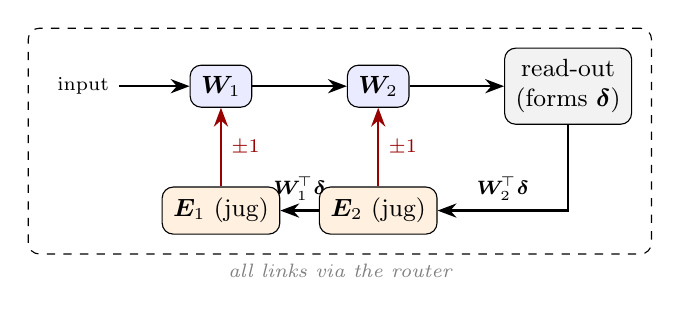
\begin{tikzpicture}[node distance=7mm and 12mm,font=\footnotesize]
  \node[ana] (w1) {$\bm W_1$};
  \node[ana,right=of w1] (w2) {$\bm W_2$};
  \node[dig,right=of w2] (ro) {read-out\\(forms $\bm\delta$)};
  \node[left=9mm of w1,font=\scriptsize] (in) {input};
  \draw[flow] (in) -- (w1);
  \draw[flow] (w1) -- (w2);
  \draw[flow] (w2) -- (ro);
  \node[jug,below=10mm of w1] (e1) {$\bm E_1$ (jug)};
  \node[jug,below=10mm of w2] (e2) {$\bm E_2$ (jug)};
  \draw[flow] (ro.south) |- (e2.east) node[near end,above,font=\scriptsize] {$\bm W_2^{\!\top}\bm\delta$};
  \draw[flow] (e2.west) -- (e1.east) node[midway,above,font=\scriptsize] {$\bm W_1^{\!\top}\bm\delta$};
  \draw[flow,red!60!black] (e1.north) -- (w1.south) node[midway,right,font=\scriptsize] {$\pm1$};
  \draw[flow,red!60!black] (e2.north) -- (w2.south) node[midway,right,font=\scriptsize] {$\pm1$};
  \begin{scope}[on background layer]
    \node[draw,dashed,rounded corners,fit=(w1)(ro)(e1)(e2)(in),inner sep=7pt,
          label={[font=\scriptsize\itshape,text=gray]below:all links via the router}] {};
  \end{scope}
\end{tikzpicture}
\caption{\textbf{The learning loop in one picture.} Forward activations pass
input $\to \bm W_1 \to \bm W_2 \to$ read-out, which forms the output error
$\bm\delta$. The error is relayed \emph{backward through the network but forward
in signalling}: each layer computes $\bm W^{\!\top}\bm\delta$ on the chip that
owns $\bm W$ and injects it into that layer's error store $\bm E$ (a leaky jug),
which writes single-code updates into $\bm W$. All links are mediated by the
router. No analog signal flows in reverse.}
\label{fig:overview}
\end{figure}

The design rests on a small set of commitments a PCN or SNN reader can
hold throughout. (i) Representation and error are separate populations
(\(\bm W\&\bm E\)). (ii) Each chip keeps exactly one copy of its weights
in SRAM and reads it three ways --- forward prediction, transpose relay,
and error accumulation. (iii) The inter-chip router only \emph{gathers}
(sum and divide); it holds no weights, so the network topology is a
soft, reconfigurable property of the router rather than fixed wiring.
(iv) All signalling is forward-directed; there is no reverse analog
channel and no counter-propagating pipeline. (v) The update approximates
the backpropagation gradient (Sec. 2), not contrastive Hebbian learning,
and is driven by a minimal global scalar --- a ``happiness'' signal
derived from the read-out's margin --- that gates learning severity
without carrying per-unit information. (vi) Every element is chosen to
be synthesisable or fabricable in an open \(130\) nm process (Sky130A).
We describe the design from the unit that matters most --- the chip and
its single weight memory --- outward to the network. Equations are
deferred to Sec. 4.

\hypertarget{the-substrate-and-its-granularity-in-hardware}{%
\subsection{The substrate and its granularity in
hardware}\label{the-substrate-and-its-granularity-in-hardware}}

The compute element, inherited from Part I \cite{dobney2026analog}, is
a five-transistor operational transconductance amplifier: an 8-bit code
held in SRAM (one step per \(1/64\) of the weight range) is converted to
a voltage on a \(200\) fF capacitor, which sets the tail current of a
differential pair and hence the transconductance by which the cell
multiplies its input. Column currents sum on a shared node by
Kirchhoff's current law, and an 8-bit SAR ADC digitises the result. The
array unit is a \(16\times16\) \emph{cell} (\(256\) such multipliers); a
\emph{chip} carries four cells; a \emph{router} mediates all traffic
between chips. Routing is performed at cell granularity and never finer,
which keeps the routing state \(O(\text{cells}^2)\) rather than
\(O(\text{synapses}^2)\); fine-grained mixing is the job of the
destination cell's own weight matrix, not of the network. Because the
router, not the wiring, defines which cell feeds which, the topology is
reconfigurable and open to experiment.

\hypertarget{the-weight-cell-is-non-linear-and-is-linearised-by-pre-distortion.}{%
\paragraph{The weight cell is non-linear, and is linearised by
pre-distortion.}\label{the-weight-cell-is-non-linear-and-is-linearised-by-pre-distortion.}}

The five-transistor cell's effective weight --- the differential-pair
transconductance --- is not linear in the stored code: it peaks near
mid-range and falls above it, so the upper half of the nominal range is
compressed and, at the extreme, inverted. This is a property of the
cell, measured across the full code range in SPICE (a
single-operating-point check cannot see it). The design linearises it in
two steps: the tail device is sized to restore monotonicity, and the
weight DAC is driven through a fixed pre-distortion table (Fig.~\ref{fig:chip}) so
that stored code maps monotonically to effective weight. With the
measured cell curve and this pre-distortion in place, accuracy is
\(81.46\%\) --- within the run-to-run noise band of the \(81.96\%\)
obtained under an ideal linear cell (Sec. 6) --- so the bit-faithful
model's linear-weight treatment is a consequence of the pre-distortion,
not an assumption.

A layer is thus \emph{factored} across chips: in the topology evaluated
here each first-layer chip maps 48 inputs to 16 outputs as three
sequential \(16\times16\) pages, and each deeper chip gathers a fixed
small number of upstream chips. This factoring is an architectural
commitment with a measurable accuracy cost, which we quantify in Sec. 6
rather than leave implicit.

\hypertarget{sec:three}{%
\subsection{One weight memory, three consumers}\label{sec:three}}

The central structural decision is that each chip holds exactly one copy
of its weights, as digital codes in a local SRAM, and that three
functionally distinct consumers read that same copy (Fig.~\ref{fig:chip}).

\begin{figure}[t]
\centering
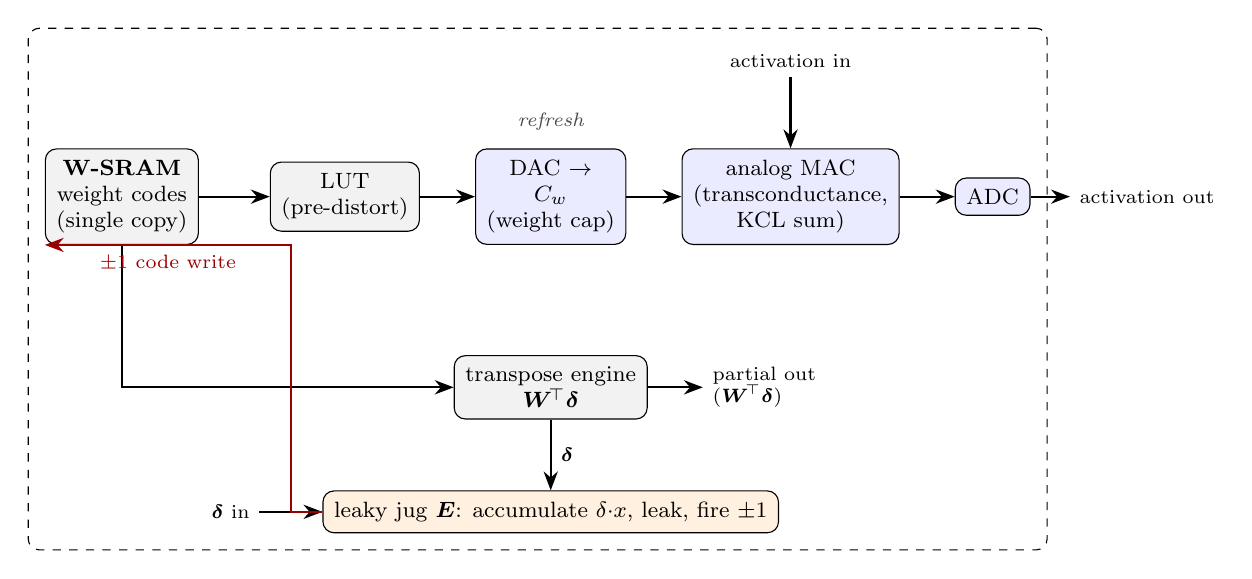
\begin{tikzpicture}[node distance=6mm and 7mm,font=\footnotesize]
  \node[dig,font=\footnotesize] (sram) {\textbf{W-SRAM}\\weight codes\\(single copy)};
  \node[dig,font=\footnotesize,right=9mm of sram] (lut) {LUT\\(pre-distort)};
  \node[ana,font=\footnotesize,right=of lut] (dac) {DAC $\to$\\$C_w$\\(weight cap)};
  \node[ana,font=\footnotesize,right=of dac] (mac) {analog MAC\\(transconductance,\\KCL sum)};
  \node[ana,font=\footnotesize,right=of mac] (adc) {ADC};
  \draw[flow] (sram) -- (lut);
  \draw[flow] (lut) -- (dac);
  \draw[flow] (dac) -- (mac);
  \node[above=1mm of dac,lbl] {refresh};
  \node[above=9mm of mac,font=\scriptsize] (ain) {activation in};
  \draw[flow] (ain) -- (mac.north);
  \draw[flow] (mac) -- (adc);
  \node[right=5mm of adc,font=\scriptsize] (aout) {activation out};
  \draw[flow] (adc) -- (aout);
  \node[dig,font=\footnotesize,below=14mm of dac] (tr) {transpose engine\\$\W^{\!\top}\bdelta$};
  \draw[flow] (sram.south) |- (tr.west);
  \node[right=7mm of tr,font=\scriptsize,align=left] (pout) {partial out\\($\W^{\!\top}\bdelta$)};
  \draw[flow] (tr) -- (pout);
  \node[jug,font=\footnotesize,below=9mm of tr] (jug)
       {leaky jug $\E$: accumulate $\delta{\cdot}x$, leak, fire $\pm1$};
  \node[left=8mm of jug,font=\scriptsize] (din) {$\bdelta$ in};
  \draw[flow] (din) -- (jug);
  \draw[flow] (tr.south) -- (jug.north) node[midway,right,font=\scriptsize] {$\bdelta$};
  \draw[flow,red!60!black] (jug.west) -- ++(-4mm,0) |- (sram.south west)
        node[near end,below,font=\scriptsize] {$\pm1$ code write};
  \begin{scope}[on background layer]
    \node[draw,dashed,rounded corners,fit=(sram)(adc)(pout)(jug)(ain),inner sep=6pt] {};
  \end{scope}
\end{tikzpicture}
\caption{\textbf{The chip: one weight memory with three consumers.} The W-SRAM (grey) is the single
copy of the weights. It drives the analog forward path (blue) through a pre-distortion LUT and a
weight DAC; it is read a second time by the on-die transpose engine, which relays error to the
preceding layer; and it is written by the leaky jug (orange), which converts accumulated error into
single $\pm1$ code steps. The incoming error $\bdelta$ is an ordinary forward-directed message and is
consumed twice, by the transpose and by the accumulator. No analog signal flows in reverse.}
\label{fig:chip}
\end{figure}

\begin{enumerate}
\def\labelenumi{\arabic{enumi}.}
\item
  \textbf{Forward prediction (\(\bm W\)).} The code is mapped through a
  pre-distortion look-up table to the weight DAC and the analog array
  multiplies the incoming activation. This is the in-memory forward
  pass.
\item
  \textbf{Backward relay (\(\bm W^{\!\top}\)).} The same codes are read
  by a small digital engine that computes \(\bm W^{\!\top}\bm\delta\)
  for the incoming error and emits the result as a partial sum. This
  digital engine could be substituted by a cross-array read as analog
  (see below).
\item
  \textbf{Error accumulation (\(\bm E\)).} The incoming error, scaled by
  the locally latched forward activity, is injected onto a per-synapse
  capacitor; a threshold crossing writes a single \(\pm1\) step back to
  the SRAM.
\end{enumerate}

Three consequences follow, and they are the reasons for the decision.
There is no second copy of any weight, hence no coherence protocol and
no weight traffic. Every quantity a weight update requires is present on
the die that owns the weight, so an update is a local transaction and
needs no global schedule (addressing the asynchrony constraint). And
because the transpose is ordinary digital arithmetic fed by a
forward-directed message, the analog array remains unidirectional
(addressing C1).

The last point deserves emphasis, because it is where the
``forwards-only'' claim could be misconstrued as bookkeeping. The claim
is physical and specific to the analog path: no current is ever driven
backwards through a transconductor, no array is bidirectional, and
nothing waits on a counter-propagating analog signal or on a switch from
a free phase to a clamped one. The digital interconnect carries typed
packets in both directions, as any network does; what
\emph{forwards-only} forbids is a reverse \emph{analog} channel, not a
reverse \emph{packet}. The error is not a backward channel but a forward
message that happens to be about the past, and decoupling it from the
forward pass in this way is what allows the signalling to be decoupled
from a clock.

\hypertarget{sec:transpose}{%
\subsection{Transpose-at-source}\label{sec:transpose}}

Mathematically, transposition is a re-indexing: summing a weight matrix
down its columns rather than across its rows. Physically, it determines
where the weights must be. There is more than one way to compute it in
an analog system. A resistive or transconductance crossbar can in
principle be driven in reverse to evaluate \(\bm W^{\!\top}\bm\delta\)
in the same array that computes the forward pass --- the analog
transpose used by some in-memory and SNN designs. We do not take this
route, because it makes the array bidirectional (C1) and couples the two
directions' operating points; instead we compute the transpose
\emph{digitally, on the chip that owns the weights}. Both are legitimate
options, and the digital choice is what keeps the analog cell strictly
one-way.

That the transpose is digital is not a concession but the design's
premise. The analog array exists for \emph{inference}, where the forward
MAC sets the power and area budget; learning is a training-time
addition. Computing \(\bm W^{\!\top}\bm\delta\) digitally --- only
during training, at 6-bit precision, on one engine time-multiplexed
across the four cells --- adds a small, amortised cost that never
touches the inference path, and in exchange keeps the analog array
strictly one-way. The question this paper answers is therefore not
\emph{analog versus digital learning} but whether an analog inference
substrate can be made to learn in place without a reverse analog
channel, a host, or a clock. Energy and area are not quantified here:
this is a pre-silicon study of the learning mechanism and its accuracy,
and a power comparison awaits the physical design.

An earlier revision of this architecture computed
\(\bm W^{\!\top}\bm\delta\) in the router, which therefore held a shadow
copy of every attached chip's weights and re-synchronised that copy
after every learning sweep. That design met the forwards-only and
asynchrony criteria in letter but not in spirit: it carried continuous
weight traffic, a coherence barrier, and a drift failure mode. Placing
the transpose on the source chip inverts the dataflow. Rather than
weights flowing outward to a computing router, the downstream error
flows inward on the existing fabric and each chip emits a finished
partial. The router retains no weights. The chip's four cells make this
efficient: one transpose engine is time-multiplexed across the cells,
amortising a single datapath over the whole die, and the engine reads
the live SRAM, so the transpose uses the current weights by construction
rather than by protocol.

One assumption is introduced. The forward pass and the subsequent
transpose may read weights that differ, because learning is continuous.
We treat this as a claim to be tested rather than argued, and measure it
in Sec. 6. Structurally it is bounded: weights change only at a periodic
sweep, and a chip's sweep cannot begin until the current batch's error
has been consumed, so the within-chip skew is zero by construction and
only cross-chip skew is at issue.

\hypertarget{sec:network}{%
\subsection{The network}\label{sec:network}}

\begin{figure}[t]
\centering
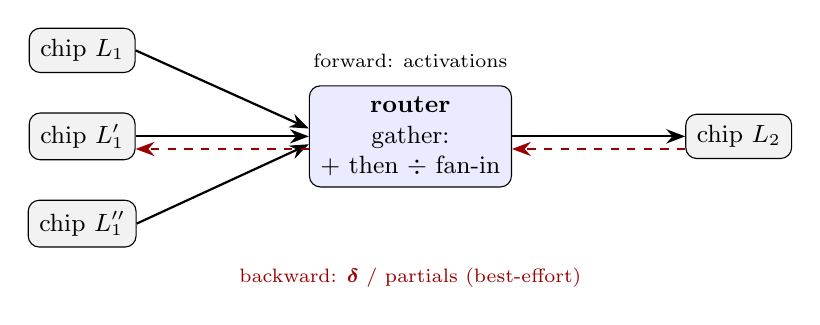
\begin{tikzpicture}[node distance=5mm and 12mm]
  \node[dig] (c1) {chip $L_1$};
  \node[dig,below=of c1] (c2) {chip $L_1'$};
  \node[dig,below=of c2] (c3) {chip $L_1''$};
  \node[ana,right=22mm of c2] (rt) {\textbf{router}\\gather:\\$+$ then $\div$ fan-in};
  \node[dig,right=22mm of rt] (d1) {chip $L_2$};
  \draw[flow] (c1.east) -- ([yshift=1mm]rt.west);
  \draw[flow] (c2.east) -- (rt.west);
  \draw[flow] (c3.east) -- ([yshift=-1mm]rt.west);
  \draw[flow] (rt.east) -- (d1.west);
  \node[above=1mm of rt,font=\scriptsize] {forward: activations};
  % backward error travels on the SAME links, drawn just below each forward arrow
  \draw[flow,dashed,red!60!black] ([yshift=-1.6mm]d1.west) -- ([yshift=-1.6mm]rt.east);
  \draw[flow,dashed,red!60!black] ([yshift=-1.6mm]rt.west) -- ([yshift=-1.6mm]c2.east);
  \node[below=9mm of rt,font=\scriptsize,text=red!60!black]
       {backward: $\bdelta$ / partials (best-effort)};
\end{tikzpicture}
\caption{\textbf{The network.} The chips perform all computation; the router only gathers. Forward
activations (solid) and error messages (dashed) share the same physical links, so there is no
separate backward network. Because the transpose runs on the chips, the router holds no weights: it
sums the partials arriving for each destination and divides by the nominal fan-in --- an adder tree
and a divider. Forward traffic is reliable; error traffic is best-effort.}
\label{fig:net}
\end{figure}

At network level (Fig.~\ref{fig:net}) the router accumulates the partials addressed
to each destination and divides by that destination's nominal fan-in.
Forward activations and error messages traverse the same physical links
in opposite directions as ordinary packets; no dedicated backward
network exists. The two message classes are given deliberately different
service guarantees, which Sec. 5 justifies. Because the router alone
determines the connectivity, changes of topology --- wider layers,
deeper stacks, alternative fan-in --- are a matter of routing
configuration rather than redesign.

\hypertarget{sec:theory}{%
\section{Formulation}\label{sec:theory}}

\hypertarget{forward-and-error-recursion}{%
\subsection{Forward and error
recursion}\label{forward-and-error-recursion}}

Write \(\bm x_0\) for the input feature vector and, for layers
\(\ell = 1,\dots,L\),
\begin{equation}
\bm a_\ell = \W_\ell \x_{\ell-1}, \qquad \x_\ell = \varphi(\bm a_\ell),
\end{equation}
with \(\varphi\) a leaky rectifier (\(\varphi(u) = u\) for \(u \ge 0\),
\(\alpha u\) otherwise, \(\alpha = 0.1\)). Each \(\bm W_\ell\) is
block-structured by the chip factoring of Sec. 3: a chip owns a set of
\(16\times16\) blocks and no block spans chips. A digital read-out
\(\bm s = \bm W_f \bm x_L + \bm b_f\) produces class scores, and the
output error for label \(y\) is
\begin{equation}
\bm e = \mathrm{onehot}(y) - \hat{\bm p},
\end{equation} \(\hat{\bm p}\) being the
read-out's class estimate. One further quantity is read from the same
scores: a scalar \emph{happiness} \(h\), the read-out's margin quantised
to a few levels (\(0\)--\(7\)), large only when a sample is
misclassified or is correct by a thin margin and zero when it is
comfortably correct. It carries no per-unit information --- one number
per sample --- and is broadcast to scale the update severity (Sec. 4.3);
pinning it to a constant recovers a fixed learning rate. The error is
then transported by the standard recursion, evaluated \emph{once} per
sample --- there is no relaxation phase, which is how C2 is discharged:
\begin{align}
\bdelta_L &= \mathcal{Q}\!\left[\,\mathcal{A}_L\!\left((\W_f^{\!\top}\bm e)\odot\varphi'(\bm a_L)\right)\right],\label{eq:dL}\\
\bdelta_{\ell-1} &= \mathcal{Q}\!\left[\,\mathcal{A}_{\ell-1}\!\left((\W_\ell^{\!\top}\bdelta_\ell)\odot\varphi'(\bm a_{\ell-1})\right)\right].\label{eq:drec}
\end{align} Equation \eqref{eq:drec} is exactly backpropagation's recursion; the
architectural content is \emph{where} each factor is evaluated. The
product \(\bm W_\ell^{\!\top}\bm\delta_\ell\) is computed on the chip
that owns \(\bm W_\ell\), from its own SRAM; the Jacobian factor
\(\varphi'(\bm a_{\ell-1})\) is a sign test on a locally latched
activation; and the sum over the chips contributing to a destination is
the router's gather. No unit needs a weight it does not own.

The two operators are the hardware. \(\mathcal{Q}\) is a fixed-range
\(b\)-bit quantiser modelling the error DAC's rails (\(b = 6\) here);
\(\mathcal{A}_\ell\) is a slow per-layer automatic gain control that
tracks the running RMS of the layer's error with an exponential moving
average and rescales to a fixed target. The AGC is not cosmetic. The
transported error attenuates by \(\approx 0.72\times\) per layer --- the
classical vanishing-gradient factor \cite{bengio1994learning}, set by
the weight norm --- so that under a \emph{fixed-range} quantiser the
error eventually underflows the LSB and \(\mathcal{Q}\) maps it
identically to zero, at which point the layer stops learning. Measured
usable depth is 4 layers without AGC and beyond 12 with it; the AGC is
what makes the quantised error path deep-scalable, and a 6-bit path with
AGC outperforms a 10-bit path without.

\hypertarget{the-update-and-why-a-naive-one-fails}{%
\subsection{The update, and why a naive one
fails}\label{the-update-and-why-a-naive-one-fails}}

The per-sample gradient contribution at layer \(\ell\) is the outer
product \(\bm g_\ell = \eta\, \bm\delta_\ell \bm x_{\ell-1}^{\!\top}\),
accumulated in the error store \(\bm E_\ell\). The question is how
\(\bm E\) is transferred to a weight cell of resolution
\(\Delta = 1/64\).

Let \(g_t\) denote the increment for one synapse at step \(t\). The
naive transfer, \(W \mathrel{+}= \mathrm{round}(g_t/\Delta)\), fails
absolutely rather than gracefully: with \(|g_t| \approx 0.019\Delta\)
the rounding returns zero for every \(t\), and the synapse never moves.
Nor is this rescued by a larger \(\eta\); Sec. 6 reports the rule to be
insensitive across a \(5\times\) range of \(\eta\). The failure is one
of \emph{resolution}, and the standard fix buys resolution with
per-synapse digital memory (the master weight of C3).

\hypertarget{sec:jug}{%
\subsection{The leaky jug as a sigma--delta modulator}\label{sec:jug}}

The alternative is to buy resolution with \emph{time}. The error store
is a capacitor \(C_e\) that is never reset. It leaks; incoming error
tops it up; and when it crosses a threshold \(\theta\) the synapse
\emph{fires}: the weight code moves by one LSB and \(\theta\) is
\emph{subtracted} from the capacitor, retaining the residue (Fig.~\ref{fig:jug}).
For one synapse, per sweep \(t\), \begin{equation}
E_t = \lambda E_{t-1} + g_t, \qquad
s_t = \operatorname{sign}(E_t)\,\mathbf{1}\!\left[|E_t| \ge \theta\right], \qquad
W_t = W_{t-1} + s_t, \qquad
E_t \leftarrow E_t - s_t\theta .
\label{eq:jug}
\end{equation}

\begin{figure}[t]
\centering
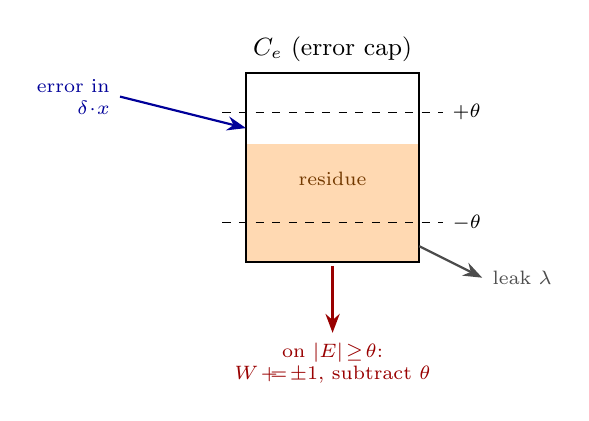
\begin{tikzpicture}[node distance=8mm]
  \fill[orange!30] (0,0) rectangle (2.2,1.5);
  \draw[thick] (0,0) rectangle (2.2,2.4);
  \node at (1.1,2.7) {\small $C_e$ (error cap)};
  \draw[dashed] (-0.3,1.9) -- (2.5,1.9) node[right,font=\scriptsize] {$+\theta$};
  \draw[dashed] (-0.3,0.5) -- (2.5,0.5) node[right,font=\scriptsize] {$-\theta$};
  \node[font=\scriptsize,text=orange!45!black] at (1.1,1.05) {residue};
  \draw[flow,blue!60!black] (-1.6,2.1) node[left,font=\scriptsize,align=right]{error in\\$\delta\!\cdot\!x$} -- (0,1.7);
  \draw[flow,gray!60!black] (2.2,0.2) -- (3.0,-0.2) node[right,font=\scriptsize,align=left]{leak $\lambda$};
  \draw[flow,red!60!black] (1.1,-0.05) -- (1.1,-0.9)
       node[below,font=\scriptsize,align=center]{on $|E|\!\ge\!\theta$:\\ $W\!\mathrel{+}\!\!=\!\pm1$, subtract $\theta$};
\end{tikzpicture}
\caption{\textbf{The leaky jug.} Error accumulates on the capacitor; it leaks, which supplies
momentum; a threshold crossing fires one weight LSB and subtracts $\theta$, retaining the residue.
The retained residue is what makes the mechanism a sigma--delta modulator rather than a lossy
quantiser.}
\label{fig:jug}
\end{figure}

The structure is a first-order sigma--delta (delta--sigma) modulator,
standard in data conversion and previously used to code activations in
neural networks \cite{oconnor2017sigma}. What is specific to this work
is its \emph{role} --- it is the weight-update path, which is what lets
a coarse analog cell learn with no per-synapse accumulator --- and the
training-specific corollaries the bounded-error property yields for the
hardware below; the modulator itself is not new.

\hypertarget{bounded-non-accumulating-quantisation-error.}{%
\paragraph{Bounded, non-accumulating quantisation
error.}\label{bounded-non-accumulating-quantisation-error.}}

Take \(\lambda = 1\) and sum \eqref{eq:jug} over \(T\) sweeps. Whatever the
comparator decides, the update to \(E\) and the update to \(W\) are the
\emph{same} event, so the identity
\begin{equation}
\theta \sum_{t=1}^{T} s_t \;=\; \sum_{t=1}^{T} g_t \;-\; E_T
\label{eq:invariant}
\end{equation} holds exactly. The left side is \(\theta\) times
the total motion of the weight code; the first term on the right is the
total accumulated gradient. Since the subtraction removes exactly
\(\theta\) whenever the level reaches \(\theta\), and the injection per
sweep is small, \(|E_T|\) remains bounded by the capacitor's clamp
\(E_{\max}\). Therefore
\begin{equation}
\Bigl| \sum_{t=1}^{T} s_t - \frac{1}{\theta}\sum_{t=1}^{T} g_t \Bigr|
\;\le\; \frac{E_{\max}}{\theta},
\label{eq:bound}
\end{equation} where \(\sum_t s_t\) is the total motion of the
weight code in LSB --- a bound \emph{independent of \(T\)}. The weight
tracks the accumulated gradient scaled by \(1/\theta\), with an error
that does not grow with the length of training. This is the sigma--delta
property, and it is the mathematical content of the design: rounding
each update discards a fixed fraction of every step (here, all of it);
the jug defers steps but discards none.

Three corollaries follow directly, and each is confirmed in Sec. 6.

\emph{\(\theta\) is the learning rate.} By \eqref{eq:bound} the weight moves
\(\sum_t g_t/\theta\) codes, so \(\theta\) sets the effective step and
is the parameter to tune. It is a comparator reference, written once at
calibration --- the same category of quantity as the ADC gain --- and is
never discovered at runtime.

\emph{The comparator may be wrong.} Identity \eqref{eq:invariant} does not assume \(s_t\)
is correct. A wrong-signed fire moves the weight the wrong way
\emph{and} pushes the residue further from zero by \(\theta\), which
makes the next fire more likely and of the correct sign; the charge is
conserved and the error is repaid. What must be accurate is the
\emph{charge on the capacitor}, not any decision made about it. This
inverts the usual analog design burden: the comparator, normally a
precision component, becomes the loose one.

\emph{Device mismatch acts as a learning-rate spread.} If \(\theta\) or
\(\lambda\) varies from synapse to synapse, \eqref{eq:bound} still holds with that
synapse's own \(\theta_i\). A leaky or high-threshold synapse does not
compute a wrong direction; it fires \emph{less often}, i.e.~it has a
smaller per-synapse learning rate. Mismatch therefore lands on the one
axis stochastic gradient descent is known to tolerate --- a random
diagonal rescaling of the step --- rather than on the gradient's sign.
Matching is consequently a non-requirement, which is unusual for an
analog array and is the property most relevant to yield. This is the
same end that in-the-loop surrogate-gradient training achieves for
spiking substrates \cite{cramer2022surrogate}, reached here without a
backward pass and with the deep credit assignment host-free (Sec. 8).

\hypertarget{one-tight-specification-and-only-one.}{%
\paragraph{One tight specification, and only
one.}\label{one-tight-specification-and-only-one.}}

The mechanism asks for analog accuracy in exactly one place: the residue
subtraction must remove a fixed charge \(\theta\) independent of the
capacitor's voltage, which is realised as a current-steered pulse
\(Q = It\). Identity \eqref{eq:invariant} is the reason it is the \emph{only} tight
specification --- because charge is conserved across the fire event,
everything downstream of it, the comparator decision included, is
permitted to be loose.

\hypertarget{the-leak-is-momentum.}{%
\paragraph{The leak is momentum.}\label{the-leak-is-momentum.}}

For \(\lambda < 1\), \eqref{eq:jug} unrolls to \(E_t = \sum_k \lambda^{t-k} g_k\),
which is the exponentially-weighted velocity of a momentum optimiser.
The capacitor's leak and the optimiser's velocity register are the same
object, so the register is not implemented but inherited. The physical
leak available is far slower than needed --- \(\approx 50\,\mu\)V/s on
\(100\) fF, i.e.~\(\approx 140\) s per error LSB, against a mean
inter-fire interval of tens of milliseconds --- so on the firing
timescale the capacitor is a pure integrator, which is the
best-performing configuration measured. The requirement is thus a loose
one-sided bound (\(\tau_{\text{leak}} \gg\) inter-fire interval,
satisfied by \(10^3\)) and not a servo.

\hypertarget{the-comparator-is-shared-and-swept-not-per-synapse.}{%
\paragraph{The comparator is shared and swept, not
per-synapse.}\label{the-comparator-is-shared-and-swept-not-per-synapse.}}

A single comparator walks the array, so a synapse is tested once per
sweep and can fire at most once per sweep. This is a design commitment
rather than an approximation: it is \(256\times\) cheaper per cell, and
the sweep period acts as a refractory interval. A per-synapse comparator
would allow repeated firing on a single crossing; we measure this to be
unstable (Sec. 6). A synapse holding \(3\theta\) therefore emits a train
of three single fires on successive sweeps rather than one triple fire
--- the boost is delayed, never discarded. Clamping the capacitor harder
would be the wrong rate limiter, as it destroys charge that \eqref{eq:invariant}
requires.

\hypertarget{the-error-is-out-of-the-forward-path.}{%
\paragraph{The error is out of the forward
path.}\label{the-error-is-out-of-the-forward-path.}}

\(C_e\) is compared, never summed into the MAC. An earlier cell placed a
second tail transistor driven by \(C_e\) so that the array computed
\(\bm W+ \bm E\). That coupling is a positive feedback loop --- error
inflates activations, which inflate errors --- and Sec. 6 shows it
degrades accuracy at the old operating point and collapses the network
beyond it. Removing it returns the cell to the original single-tail
topology and dissolves a biasing constraint, so the simulator and the
silicon compute the same function.

\hypertarget{sec:interconnect}{%
\section{Interconnect and asynchrony}\label{sec:interconnect}}

The message classes are given different guarantees, and the asymmetry is
earned rather than assumed. Forward activations are delivered
\emph{reliably}, because a forward pass needs its complete input vector.
Error messages and transpose partials are \emph{best-effort}: they are
fired into accumulators, and a dropped partial contributes zero.
Equation \eqref{eq:invariant} is what licenses this --- a lost or late error under-fills
a jug that self-corrects over subsequent sweeps, whereas a lost
activation corrupts a prediction irrecoverably.

This is where C4 is discharged in practice. The interconnect carries
typed messages, and the type --- graded packet, event, or spike --- is a
property of the fabric, not of the learning rule; a spiking link and a
graded-packet link are interchangeable as far as \eqref{eq:invariant} is concerned, since
all the jug requires is that charge arriving over time be conserved.

What makes the fabric clock-free is a single structural fact: the gather
is a sum, and addition commutes, so partials may arrive in any order.
The router therefore divides by the destination's \emph{nominal} fan-in
when the batch tag closes and forwards the result, rather than waiting
for every contributor.

A wait-for-all barrier is a distributed synchronisation primitive and
was the last one in the design; fixed-divide removes it, at the cost of
slightly under-driving an error when a partial is missing --- the
tolerated failure mode above. Batch grouping reuses the existing 4-bit
sequence field so that partials from different batches cannot blend, and
a configurable freshness window (default four batches) bounds buffering.

Within the window the policy is to apply late rather than drop, since a
dropped error loses a gradient whereas a late error costs only bounded
skew --- and Sec. 6 shows that cost to be small. A loose default matters
because the fabric is heterogeneous: nodes on different process nodes
run at different rates, and a tight window would penalise the slower
node on every batch.

\hypertarget{sec:results}{%
\section{Evaluation}\label{sec:results}}

\hypertarget{method}{%
\subsection{Method}\label{method}}

Evidence is organised as three levels, each constraining the one above:
Python behaviour (does the rule learn?), Sky130A SPICE (does the analog
physics permit it?), and RTL (does the digital realisation reproduce the
arithmetic?). The behavioural rig is reported here; the design has
additionally been carried to Sky130A SPICE and to a bit-faithful RTL
implementation, whose netlists, listings, and test benches are in the
repository, and we draw on those levels only where a specific claim
depends on them.

Two Python rigs are used and are kept distinct. A \emph{float} reference
implements the topology and the rule in floating point and is not
modified for experiments. A \emph{bit-faithful} model quantises the
weight cell, the activations, the error path, and the update, and
carries the jug. Each rig is reported against its own control, and
figures from different rigs are never compared.

One scope note. The linear read-out \((\bm W_f, \bm b_f)\) is fit by a
host least-squares step --- L-BFGS logistic regression for the final
reported number --- on the learned features; it is a single-layer
classifier on fixed features, not an in-the-loop gradient through the
network. Every hidden-layer weight update, which is the subject of this
paper, is performed by the on-die rule with no host. Where we say
``host-free'' below we mean this deep credit assignment; the final
read-out is host-fit, as is standard for evaluating learned features.

The task is EMNIST letters \cite{cohen2017emnist} (26 classes, full
test set). The topology, denoted BIG, is 48 chips: \(1152\) input
features (split-sign encoded) \(\to\) \(384\) \(\to\) \(128\) \(\to\)
\(256\), with a digital read-out. Run-to-run spread at the working
operating point is \(0.7\) percentage points (pp), measured over four
seeds; we treat differences within that band as indistinguishable and
say so where it matters.

\hypertarget{does-the-forwards-only-rule-learn}{%
\subsection{Does the forwards-only rule
learn?}\label{does-the-forwards-only-rule-learn}}

Table 1 reports the primary result. The forwards-only rule, carrying
every hardware constraint simultaneously (6-bit error broadcast,
severity-gated read-out error, 4-bit error integrator, 1-bit sign write
at the fold, 8-bit weight rail), reaches \(82.50\%\). The comparison
that matters is against full backpropagation on the \emph{identical}
chip-factored topology with the same 8-bit weight rail, trained with
signed SGD and momentum in an independent framework: \(82.85\%\). The
gap is \(0.35\) pp, within the noise band. On this topology the
learning-rule question is therefore closed: the constraints cost
essentially nothing.

Two further rows are needed to read that number honestly. A linear
classifier on the same \(1152\) input features reaches \(77.14\%\), so
the network is contributing \(5.4\) pp of genuine nonlinear learning
rather than inheriting its accuracy from the features. And the same
backpropagation reference on a \emph{dense} network of identical widths
reaches \(89.48\%\): the \(6.6\) pp difference is the price of chip
factoring --- of forbidding cross-chip mixing within a layer --- and is
the largest single deficit remaining in the design. It is a question of
width and connectivity --- topology, not of the learning rule, and it is
the subject of ongoing work.

\begin{longtable}[]{@{}
  >{\raggedright\arraybackslash}p{(\columnwidth - 2\tabcolsep) * \real{0.8537}}
  >{\raggedleft\arraybackslash}p{(\columnwidth - 2\tabcolsep) * \real{0.1463}}@{}}
\caption{Learning rule, float rig, EMNIST letters, BIG
topology.}\tabularnewline
\toprule\noalign{}
\begin{minipage}[b]{\linewidth}\raggedright
Configuration
\end{minipage} & \begin{minipage}[b]{\linewidth}\raggedleft
Accuracy
\end{minipage} \\
\midrule\noalign{}
\endfirsthead
\toprule\noalign{}
\begin{minipage}[b]{\linewidth}\raggedright
Configuration
\end{minipage} & \begin{minipage}[b]{\linewidth}\raggedleft
Accuracy
\end{minipage} \\
\midrule\noalign{}
\endhead
\bottomrule\noalign{}
\endlastfoot
Backpropagation, dense network, same widths & 89.48\% \\
Backpropagation, chip-factored \(+\) 8-bit rail (signSGD \(+\) momentum)
& \textbf{82.85\%} \\
\textbf{Forwards-only rule, all hardware constraints} &
\textbf{82.50\%} \\
Forwards-only rule, unconstrained error broadcast & 82.89\% \\
Linear classifier on the \(1152\) input features (baseline) & 77.14\% \\
Prior rule (fold/absorb), best of an extended search & 64.09\% \\
\end{longtable}

\hypertarget{does-the-rule-survive-the-hardware-arithmetic}{%
\subsection{Does the rule survive the hardware
arithmetic?}\label{does-the-rule-survive-the-hardware-arithmetic}}

Carried onto a bit-faithful model --- the same rule with the weight
cell, activations, error path, and update all quantised and the jug in
place --- accuracy is \(81.96\%\) against a floating-point ceiling of
\(82.13\%\) for that model (with the measured weight-cell curve and
pre-distortion in place, \(81.46\%\); Sec. 3.2). The move to hardware
arithmetic therefore costs \(0.17\) pp, a quarter of the noise band, and
it does so while \emph{deleting} the digital master weight, the velocity
register, and all per-synapse digital state that a conventional sub-LSB
accumulator (C3) would require. A naive write of the same rule to the
8-bit cell, by contrast, reaches only \(75.25\%\): the sigma--delta
mechanism, not extra learning rate, is what closes the gap --- the
working configuration fires on only \(0.91\%\) of synapse-sweeps --- and
\(\theta\) behaves as the effective learning rate that \eqref{eq:bound} predicts.

\hypertarget{robustness}{%
\subsection{Robustness}\label{robustness}}

Table 2 tests the three corollaries of Sec. 4.3 against deliberately
hostile device models. Leakage was modelled as log-normal per synapse
(subthreshold leakage is exponential in threshold voltage, whose
mismatch is Gaussian), drawn once as fabrication rather than noise. At
\(\tau = 100\) folds with a \(3\times\) spread the median synapse drains
about as fast as it fills and the worst \(5\%\) leak six times faster
than they fire; the cost is \(0.43\) pp.~A \(10\times\) spread costs
\(0.58\) pp.~Doubling the spread of \(\theta\) costs \(0.76\) pp.~Every
figure is at or near the noise band, as \eqref{eq:bound} predicts, because each
perturbation is a per-synapse learning rate rather than a corrupted
direction. The frozen fraction rises substantially (from \(35\%\) to
\(66\%\) at \(\tau=100\)) and accuracy holds regardless: the network
does not need every synapse, only those with evidence.

The comparator result is the sharpest test of the theory. Forcing the
fire decision to take the wrong sign on \(20\%\) of crossings costs
\(0.34\) pp.~A component allowed a one-in-five error rate is not a
precision component, and this is a direct consequence of identity \eqref{eq:invariant}
rather than a fortunate empirical finding.

A counter-test of allowing the error capacitor to contribute to the
forward MAC costs \(1.5\) pp at the former design point and collapses
the network entirely (\(47 \to 12\%\)) at twice that coupling, with the
firing rate running away to \(19.3\%\) per fold; this is why the cell is
single-tail. Permitting multiple fires per crossing (a per-synapse
comparator) drives the firing rate to \(271\%\) per fold and collapses
accuracy to \(18\%\); this is why the comparator is swept.

\begin{longtable}[]{@{}
  >{\raggedright\arraybackslash}p{(\columnwidth - 4\tabcolsep) * \real{0.4833}}
  >{\raggedleft\arraybackslash}p{(\columnwidth - 4\tabcolsep) * \real{0.4500}}
  >{\raggedleft\arraybackslash}p{(\columnwidth - 4\tabcolsep) * \real{0.0667}}@{}}
\caption{Robustness of the jug (bit-faithful rig, BIG). Clean reference
\(81.96\%\); noise band \(0.7\) pp.}\tabularnewline
\toprule\noalign{}
\begin{minipage}[b]{\linewidth}\raggedright
Perturbation
\end{minipage} & \begin{minipage}[b]{\linewidth}\raggedleft
Accuracy
\end{minipage} & \begin{minipage}[b]{\linewidth}\raggedleft
Cost
\end{minipage} \\
\midrule\noalign{}
\endfirsthead
\toprule\noalign{}
\begin{minipage}[b]{\linewidth}\raggedright
Perturbation
\end{minipage} & \begin{minipage}[b]{\linewidth}\raggedleft
Accuracy
\end{minipage} & \begin{minipage}[b]{\linewidth}\raggedleft
Cost
\end{minipage} \\
\midrule\noalign{}
\endhead
\bottomrule\noalign{}
\endlastfoot
None (clean devices) & 81.96\% & --- \\
Leakage \(\tau = 1000\) folds, \(3\times\) log-normal spread & 81.68\% &
\(0.28\) \\
Leakage \(\tau = 100\) folds, \(3\times\) spread & 81.53\% & \(0.43\) \\
Leakage \(\tau = 1000\) folds, \(10\times\) spread & 81.38\% &
\(0.58\) \\
Threshold \(\theta\) mismatch \(\times 2\) & 81.20\% & \(0.76\) \\
Comparator sign wrong on \(20\%\) of fires & 81.62\% & \(0.34\) \\
Seeds (\(n=4\)) & \(81.38\) / \(81.63\) / \(81.96\) / \(82.17\) (mean
\(81.79\)) & \\
\end{longtable}

\hypertarget{robustness-in-the-face-of-asynchronicity}{%
\subsection{Robustness in the face of
asynchronicity}\label{robustness-in-the-face-of-asynchronicity}}

Sec. 3.4 introduced one load-bearing assumption: that the forward pass
and the transpose may read different weights. We tested it directly by
forcing the transpose to read weights staled by \(k\) update batches
(Table 3). A one-batch skew --- the realistic worst case, since a chip's
sweep cannot precede the consumption of that batch's error --- is free
at two convergence levels. The penalty for gross violations is bounded
and does not grow with \(k\): \(k = 2, 4, 8\) are mutually
indistinguishable within the noise band, and uncorrelated staleness at
\(k = 8\) costs \(0.34\) pp.~This is consistent with the transported
error being a \emph{direction} generator feeding a slow charge
accumulator, and with an independent probe finding the cosine similarity
to the true gradient statistically unchanged by weight drift (\(0.980\)
with, \(0.973\) without). Temporal skew is not a blocker, and the
freshness window may accordingly be set loose.

\begin{longtable}[]{@{}
  >{\raggedright\arraybackslash}p{(\columnwidth - 12\tabcolsep) * \real{0.2597}}
  >{\raggedleft\arraybackslash}p{(\columnwidth - 12\tabcolsep) * \real{0.0909}}
  >{\raggedleft\arraybackslash}p{(\columnwidth - 12\tabcolsep) * \real{0.1429}}
  >{\raggedleft\arraybackslash}p{(\columnwidth - 12\tabcolsep) * \real{0.0909}}
  >{\raggedleft\arraybackslash}p{(\columnwidth - 12\tabcolsep) * \real{0.0909}}
  >{\raggedleft\arraybackslash}p{(\columnwidth - 12\tabcolsep) * \real{0.0909}}
  >{\raggedleft\arraybackslash}p{(\columnwidth - 12\tabcolsep) * \real{0.2338}}@{}}
\caption{Forward/transpose weight skew, in update batches
(float-topology rig; two convergence levels). \(k=1\) is the realistic
bound.}\tabularnewline
\toprule\noalign{}
\begin{minipage}[b]{\linewidth}\raggedright
Skew \(k\) (batches)
\end{minipage} & \begin{minipage}[b]{\linewidth}\raggedleft
0
\end{minipage} & \begin{minipage}[b]{\linewidth}\raggedleft
1
\end{minipage} & \begin{minipage}[b]{\linewidth}\raggedleft
2
\end{minipage} & \begin{minipage}[b]{\linewidth}\raggedleft
4
\end{minipage} & \begin{minipage}[b]{\linewidth}\raggedleft
8
\end{minipage} & \begin{minipage}[b]{\linewidth}\raggedleft
8 (uncorrelated)
\end{minipage} \\
\midrule\noalign{}
\endfirsthead
\toprule\noalign{}
\begin{minipage}[b]{\linewidth}\raggedright
Skew \(k\) (batches)
\end{minipage} & \begin{minipage}[b]{\linewidth}\raggedleft
0
\end{minipage} & \begin{minipage}[b]{\linewidth}\raggedleft
1
\end{minipage} & \begin{minipage}[b]{\linewidth}\raggedleft
2
\end{minipage} & \begin{minipage}[b]{\linewidth}\raggedleft
4
\end{minipage} & \begin{minipage}[b]{\linewidth}\raggedleft
8
\end{minipage} & \begin{minipage}[b]{\linewidth}\raggedleft
8 (uncorrelated)
\end{minipage} \\
\midrule\noalign{}
\endhead
\bottomrule\noalign{}
\endlastfoot
Accuracy (early) & 67.47 & \textbf{67.47} & 66.33 & 65.75 & 66.34 &
67.13 \\
Accuracy (later) & 72.43 & \textbf{72.43} & 71.00 & --- & --- & --- \\
\end{longtable}

\hypertarget{does-the-analog-physics-permit-it-spice}{%
\subsection{Does the analog physics permit it?
(SPICE)}\label{does-the-analog-physics-permit-it-spice}}

Two transistor-level results support the design's central claims, and
both concern the one place the mechanism is demanding. First, the
residue subtraction of \eqref{eq:jug} is realised as a current-steered charge
pulse, \(Q = It\), and is verified in Sky130A SPICE to remove a
\emph{fixed} charge independent of the capacitor's voltage. This is the
design's single tight analog specification, and identity \eqref{eq:invariant} is the
reason it is the only one: because charge is conserved across the fire
event, everything downstream of it is permitted to be loose. Second, the
component the theory allows to be loose --- the comparator --- is, in
silicon, comfortably precise: a transistor-level window comparator
settles to within \(0.75\) mV of each threshold, with a dead zone of
\(\approx 0.2\,\mu\)V, in \(2.5\) ns. The robustness measurement above
shows the sigma--delta absorbs \emph{wrong} comparator decisions at the
level of tens of percent; the physical comparator errs at the level of
microvolts. The tolerance the theory demands and the margin the physics
delivers are therefore separated by orders of magnitude. (A bit-faithful
RTL realisation independently reproduces the transpose within \(\pm1\)
LSB and every residue of \eqref{eq:jug} within \(2\,\mu\)V of the model; netlists
and test benches are in the repository.)

\hypertarget{sec:history}{%
\section{Design history and negative results}\label{sec:history}}

The design's history is reported because several of its dead ends are
informative and two of them are methodological.

\hypertarget{bidirectional-schemes-were-abandoned-first.}{%
\paragraph{Bidirectional schemes were abandoned
first.}\label{bidirectional-schemes-were-abandoned-first.}}

The work began with a contrastive Hebbian arrangement in which each chip
exchanged signals in both directions with its parent. It functioned, but
pipelining data in two directions forced a central clock and a
management layer to keep the directions aligned --- an arrangement that
becomes harder, not easier, as clock distribution degrades across a
growing fabric and represented increasing fragility and parameter
sensitivity in the design. This is C1 and C2 of Sec. 2.2 met head-on,
and it is what produced the forwards-only and asynchrony constraints as
invariants rather than preferences.

\hypertarget{a-long-plateau-under-a-bm-wbm-e-decomposition.}{%
\paragraph{\texorpdfstring{A long plateau under a \(\bm W{+}\bm E\)
decomposition.}{A long plateau under a \textbackslash bm W\{+\}\textbackslash bm E decomposition.}}\label{a-long-plateau-under-a-bm-wbm-e-decomposition.}}

The first forwards-only learning scheme started with a more modular W+E
design that kept weights \(\bm W\) and an error store \(\bm E\) per
chip, updating \(\bm E\) per sample and folding it into \(\bm W\)
periodically. We explored it extensively --- two- and three-layer
topologies, frozen and staged training, and a range of feedback signals
including a deliberately minimal global scalar that still supports
learning. It learned, but repeatedly stalled near \(64\%\): freezing one
layer inhibited others, and error routed around the \(\bm W{+}\bm E\)
loop tended toward wrong directions or oscillation. The reversals had
identifiable causes --- a non-stationary objective, since the read-out
was refit each epoch; fixed-magnitude sign steps, which orbit rather
than converge; and training only on misclassified samples, which starves
as the baseline improves.

\hypertarget{on-method.}{%
\paragraph{On method.}\label{on-method.}}

The hardware gap was ultimately closed by elimination rather than
hypothesis. Every quantiser was ablated individually and each was
innocent --- weight cell \(0.4\) pp, ADC \(0\), error channel \(0\),
error accumulator \(0\) --- which appeared to be failure and was not: it
identified the update path, the one component never isolated. For
instance, hypotheses chosen because they were plausible (crest factor,
ADC width, analog cell precision) were all wrong in practice or required
over-complex hardware. The `leaky-jug' accumulator was discovered
because other options failed.

\hypertarget{sec:related}{%
\section{Related work and positioning}\label{sec:related}}

The design sits between three lines of analog-learning research, and is
best understood by what it takes from each and what it refuses.

\hypertarget{analog-in-memory-training-on-non-volatile-memory.}{%
\paragraph{Analog in-memory training on non-volatile
memory.}\label{analog-in-memory-training-on-non-volatile-memory.}}

Training in analog memory arrays has reached digital-equivalent accuracy
\cite{ambrogio2018equivalent}, but it runs conventional backpropagation
--- including the transposed backward pass we avoid --- and leans on
device-level symmetry of the weight update. A related line, resistive
processing units \cite{gokmen2016acceleration}, makes exactly the
digital-accumulator-and-periodic-transfer choice we identify as C3's
master weight, and carries its per-synapse memory cost. The sigma--delta
update relaxes exactly that requirement: because \eqref{eq:invariant} conserves charge
across an imperfect comparator, the write need not be symmetric or
linear, only charge-conserving. Our low firing rate (\(0.91\%\) of
synapse-sweeps) also bears on endurance-limited memories, since it
reduces write traffic by orders of magnitude relative to
update-every-step schemes, though we make no density claim: an analog
capacitor is larger than an SRAM byte, and this substrate does not
compete on weight density. The strength here is the rule itself: it is
not tied to this substrate, and can be applied to other analog cells or
even a purely digital accumulator.

\hypertarget{mixed-signal-spiking-neuromorphic-systems.}{%
\paragraph{Mixed-signal spiking neuromorphic
systems.}\label{mixed-signal-spiking-neuromorphic-systems.}}

The SNN tradition shares our substrate premise --- compute as analog
sums, communicate as digital events
\cite{cramer2022surrogate, chicca2014neuromorphic, benjamin2014neurogrid, moradi2018dynap};
our C4 (Sec. 2) is precisely that the second half of that premise is a
communication choice, not a computational one, and here the error
travels forward only, with the hidden-layer learning host-free. On-chip
local rules that do dispense with the host
\cite{rubino2023neuromorphic} remain Hebbian or spike-timing based and,
like the on-chip plasticity of Loihi \cite{davies2018loihi}, do not
reach backpropagation-grade credit assignment on deep tasks; the
forwards-only rule does, on this topology, at the cost only of chip
factoring.

\hypertarget{predictive-coding-and-feedback-alignment.}{%
\paragraph{Predictive coding and feedback
alignment.}\label{predictive-coding-and-feedback-alignment.}}

Within PC, Whittington and Bogacz \cite{whittington2017approximation}
establish the backpropagation relationship the rule relies on, and
synthesisable digital PC networks have been reported
\cite{oh2026synthesizable}; our aim differs in that the arithmetic is
analog and in-memory by construction and the digital logic exists only
to move and accumulate error. Feedback alignment and its direct variant
\cite{lillicrap2016random, nokland2016direct} solve the
weight-transport problem by discarding the transpose in favour of fixed
random feedback --- a legitimate and arguably cheaper answer to C1, and
one compatible with this fabric. We retain the true transpose because
transpose-at-source makes it \emph{free of transport}: the weights are
already on the die that needs them, so the accuracy risk of a random
feedback path buys nothing here. A direct comparison on this substrate
is future work. Equilibrium propagation \cite{scellier2017equilibrium},
another local rule that approximates backpropagation, is a natural
analog candidate but reintroduces the iterative relaxation (C2) this
design abandons.

\hypertarget{sec:conclusion}{%
\section{Limitations and conclusion}\label{sec:conclusion}}

\hypertarget{limitations.}{%
\paragraph{Limitations.}\label{limitations.}}

All results are pre-silicon: Python, SPICE and RTL, not a fabricated
die. The largest known accuracy deficit is not the learning rule but the
chip factoring, which costs \(6.6\) pp against a dense network of the
same widths (Table 1); widening the fabric is the obvious lever and is
untested at scale under the current rule. The jug's threshold is
evaluated on a batch grid in simulation, whereas the hardware evaluates
it per sweep; a per-sample leak model is required before a circuit
specification is frozen. We have modelled static device mismatch but not
thermal drift during training. The weight capacitor's own leakage is
treated by SRAM refresh, and the inter-chip protocol is specified but
not yet realised across the heterogeneous process nodes the architecture
anticipates. The supervised rule is evaluated on a single task (EMNIST
letters) with a linear read-out --- Part I established the substrate on
MNIST and EMNIST under unsupervised feature learning
\cite{dobney2026analog}, but the supervised rule here is characterised
on one dataset only; its behaviour on harder problems --- in particular
whether the momentum the leak supplies earns its keep, which it does not
measurably do here --- is open.

\hypertarget{conclusion.}{%
\paragraph{Conclusion.}\label{conclusion.}}

We have described an analog predictive-coding substrate that can be
trained in place under three constraints usually treated as obstacles:
no calibration, no reverse signal path, no global clock. The design
reduces to a small, self-contained predictive-coding level in a W\&E
design --- weights held as capacitor charge with SRAM refresh, an error
capacitor whose threshold crossings adjust those weights by one code at
a time, and a local transpose that relays error to the level below. Its
two enabling ideas are independent of this substrate and may be of wider
use. Computing the transpose at the source removes the weight copy, and
with it the coherence and synchronisation the copy demands. And the
sigma--delta update converts training from a problem of \emph{precision}
into a problem of \emph{time} --- fire occasionally and conserve charge
--- which is the trade a capacitor makes naturally, and which leaves the
comparator free to be wrong. Against the mixed-signal SNN systems this
substrate is adjacent to, the distinction is not that it tolerates
mismatch --- adaptive analog learning already does --- but that it
reaches backpropagation-grade accuracy with the error travelling forward
only, the deep credit assignment host-free (only the final linear
read-out is host-fit), and no global clock. Under these mechanisms a
forwards-only network of such chips learns as well as backpropagation on
the same topology, while every weight stays where it is.

\hypertarget{acknowledgements}{%
\section*{Acknowledgements}\label{acknowledgements}}
\addcontentsline{toc}{section}{Acknowledgements}

Architectural direction and design decisions are the author's. The
simulators, SPICE netlists, and RTL were implemented with Claude Code
\cite{anthropic2025claudecode} (Opus and Fable models), whose
contribution was the rate at which code and tests could be produced to
explore the topology, algorithm, and parameter space and to characterise
the physics.


\bibliographystyle{IEEEtran}
\bibliography{refs}
\end{document}
